\section{Data}
\label{sec:data}

This study focuses on stellar rotation in the original \kepler\ field.
This is partly because \kepler\ provides the largest sample of published,
homogeneously measured rotation periods, and partly because its low Galactic
latitude allows us to marginalize over missing RV measurements and approximate
vertical velocity, \vz.

We combined two large rotation period catalogs constructed from original
\kepler\ data, from \citet{mcquillan2014} and \citet{santos2019}.
These two studies used different techniques to measure rotation periods from
\kepler\ light curves: autocorrelation functions and wavelets respectively.
The \citet{santos2019} study was specifically focused on cooler stars: K and M
dwarfs, and includes a larger number of rotation periods for these stars.
The combined catalogs provide a total of over 38,000 rotation periods.

\begin{itemize}
    \item{Describe cuts and Gaia crossmatch.}
    \item{Reddening calculation.}
    \item{Photometric temperatures.}
    \item{Binary and subgiant cuts?}
    \item{Gyro age cuts?}
    \item{Radial velocity replacement.}
    \item{Velocity calculation.}
\end{itemize}

To calculate kinematic ages, an estimate of vertical velocity, \vz, is
required.
The ideal way to calculated \vz\, and similarly, \vx\ and \vy, is to use 6D
positional and velocity information.
Many stars in the \kepler\ field do not have RV measurements and an
alternative approach must be taken to infer their vertical velocities (see
section \ref{sec:velocity_inference}).
However, a large number of \kepler\ rotators, over 10,000 of 34,000 {\it do}
have RV measurements from \gaia\ DR2 and \lamost.
Figure \ref{fig:existing_rvs} shows rotation period vs effective temperature
for all stars in the \mct\ and \citet{santos2019} catalogs, plotted in grey.
Stars with RV measurements are colored by their vertical velocity dispersion
(see section \ref{sec:velocity_dispersion} to see how we calculated velocity
dispersion).
\racomment{Discuss what this plot shows}.

Although RVs are available for a significant number of \kepler\ rotators
(almost one in three), few stars cooler than 4000 K have RV measurements.
This is due to the faint limits of the \gaia\ DR2 and \lamost\ surveys
(although RV measurements for fainter targets will be available in \gaia\
DR3).
Given that magneto-rotational evolution is poorly understood for M dwarfs, the
cool stars with missing RVs are arguably the ones we care most about.
For this reason, we attempted to compensate for the lack of RV measurements by
inferring vertical velocities for stars without RVs, to fill in the
low-temperature region of figure \ref{fig:existing_rvs} in section
\ref{sec:velocity_inference}.
\begin{figure}[ht!]
\caption{
Vertical velocity dispersion as a function of rotation period and effective
    temperature for \kepler\ stars with measured rotation periods.
Colored points show stars with RV measurements from \gaia\ or \lamost, with
    their color indicating their velocity dispersion.
Faint grey points show the combined \mct\ and \citet{santos2019} samples,
    including stars without RV measurements.
The coolest stars in this sample do not have RVs because they are faint.
}
  \centering 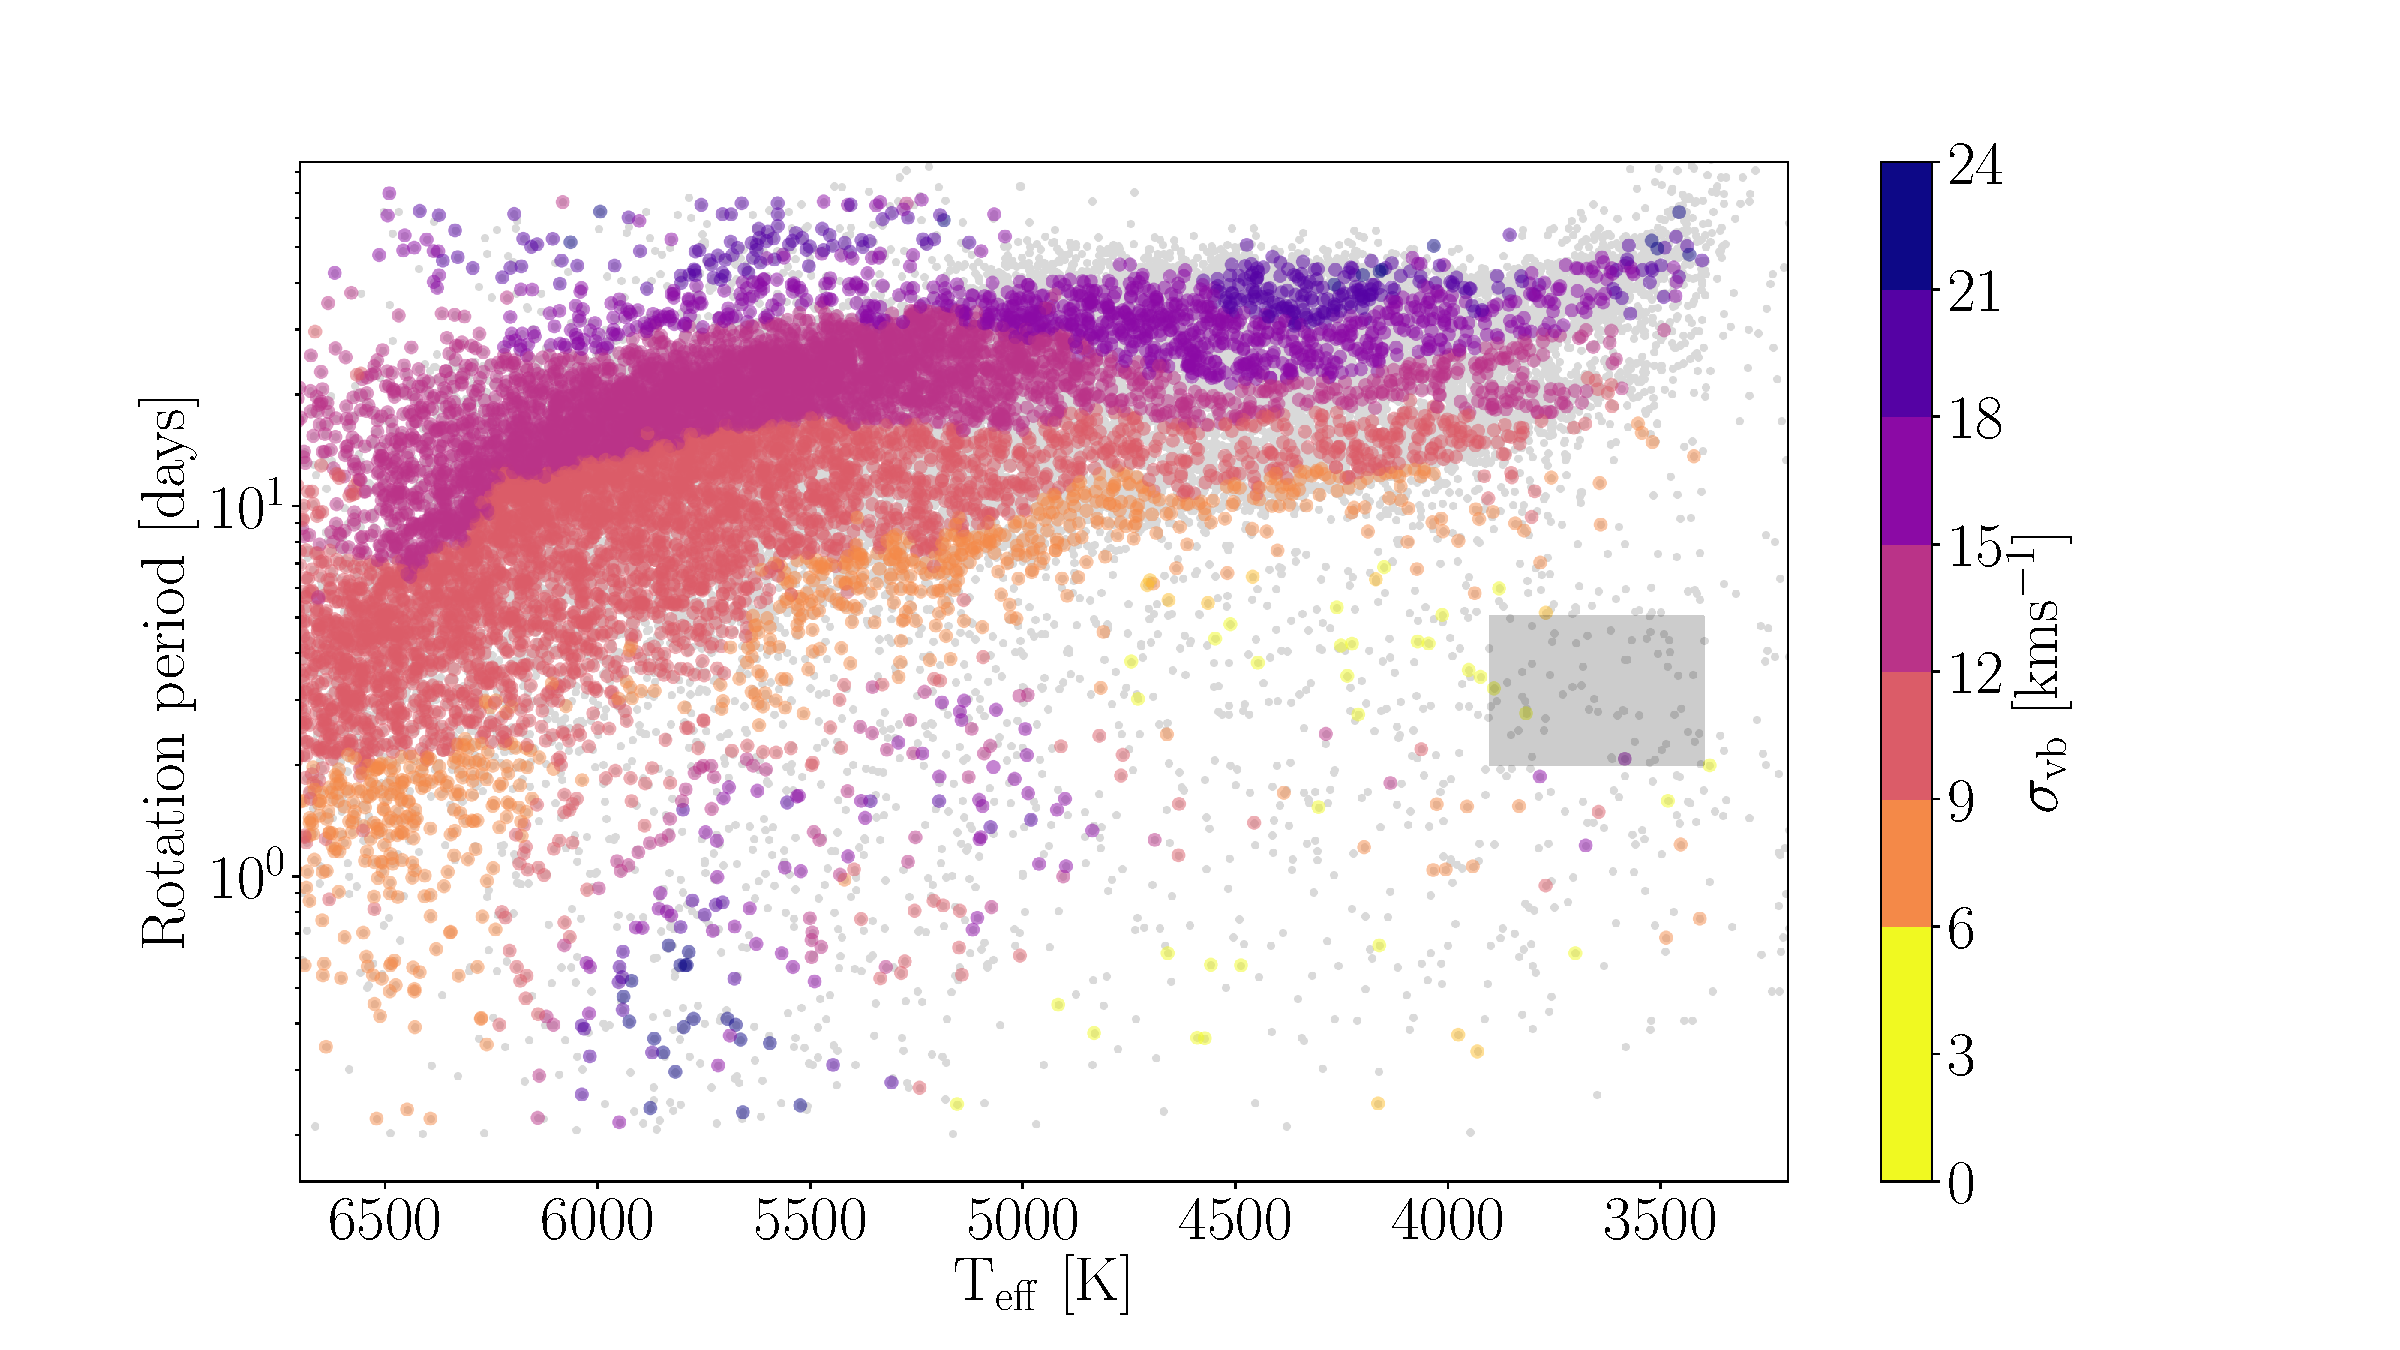
\includegraphics[width=1\textwidth]{existing_rvs}
\label{fig:existing_rvs}
\end{figure}

